%%%%%%%%%%%%%%%%%%%% author.tex %%%%%%%%%%%%%%%%%%%%%%%%%%%%%%%%%%%
%
% sample root file for your "contribution" to a contributed volume
%
% Use this file as a template for your own input.
%
%%%%%%%%%%%%%%%% Springer %%%%%%%%%%%%%%%%%%%%%%%%%%%%%%%%%%


% RECOMMENDED %%%%%%%%%%%%%%%%%%%%%%%%%%%%%%%%%%%%%%%%%%%%%%%%%%%
\documentclass[graybox]{svmult}

% choose options for [] as required from the list
% in the Reference Guide

\usepackage{mathptmx}       % selects Times Roman as basic font
\usepackage{helvet}         % selects Helvetica as sans-serif font
\usepackage{courier}        % selects Courier as typewriter font
\usepackage{type1cm}        % activate if the above 3 fonts are
                            % not available on your system
%
\usepackage{makeidx}         % allows index generation
\usepackage{graphicx}        % standard LaTeX graphics tool
                             % when including figure files
\usepackage{multicol}        % used for the two-column index
\usepackage[bottom]{footmisc}% places footnotes at page bottom

\usepackage[sort&compress,numbers]{natbib}
\usepackage{todonotes}

%% macros for the manuscript.... %%%%%%%%%%%%%%%%%%%%%%%%%%%%%%%%%%%%%%%%%%%

\renewcommand{\lhd}{\ensuremath{\mathcal{L}}}
\newcommand{\intd}{\ensuremath{\mathrm{\;d\,}}}


%%%%%%%%%%%%%%%%%%%%%%%%%%%%%%%%%%%%%%%%%%%%%%%%%%%%%%%%%%%%%%%%%%%%%%%%%


% see the list of further useful packages
% in the Reference Guide

\makeindex             % used for the subject index
                       % please use the style svind.ist with
                       % your makeindex program

%%%%%%%%%%%%%%%%%%%%%%%%%%%%%%%%%%%%%%%%%%%%%%%%%%%%%%%%%%%%%%%%%%%%%%%%%%%%%%%%%%%%%%%%%

\begin{document}

\title*{Ancestral population genomics with Jocx, a coalescent hidden Markov model}
\author{Jade Yu Cheng and Thomas Mailund}
\institute{Jade Yu Cheng \at FIXME
	\email{name@email.address}
\and Thomas Mailund \at Bioinformatics Research Centre, Aarhus University \email{mailund@birc.au.dk}}
\maketitle

\abstract{FIXME}


\section{Introduction}

\todo[inline]{Stuff we need to include: 1) Which models can Jocx analyse and how? 2) Description of the data we put on GitHub, 3) Simulation results for the models we present, showing how Jocx does on those---probably with scripts (on GitHub) for making the plots}


Understanding how species form and diverge is a central topic of biology and by observing emerging species today we can understand many of the genetic and environmental processes involved. Through such observations we can understand the underlying forces that drive speciation, but in order to understand how specific speciations occurred in the past, and understand the specifics of how existing species formed, we must make inference from the signals these events have left behind. The study of fossils is a powerful approach here, but not the only avenue to study past speciations; the speciation processes leave fossils in the genome of the resulting species, and through what you might call genetic archaeology we can study past events from the signals they left behind.


The main objectives of the methods we describe in this chapter is to infer demographic parameters, $\Theta$, given genetic data, $D$: $\lhd(\Theta\,|\,D)=\Pr(D\,|\,\Theta)$. Here, we assume that $\Theta$ contains information such as effective population sizes, time points where population structure changes (populations split or admix), or migration rates between populations. We can connect data and demographics through coalescence theory \cite{Hein:2004ta}. This theory gives us a way to assign probability densities to genealogies, densities that depend on the demographic parameters, $f(G\,|\,\Theta)$. Then, if we know the underlying genealogy, we can assign probabilities to observed data using standard algorithms such as \citet{Felsenstein_1981} and get $\Pr(D\,|\,G,\Theta)$. Theoretically, we now simply need to integrate away the nuisance parameter $G$ to get the desired likelihood
\begin{equation}
	\label{eq:likelihood}
	\lhd(\Theta\,|\,D) = \Pr(D\,|\,\Theta)
	= \int \Pr(D\,|\,G,\Theta) f(G\,|\,\Theta) \intd G .
\end{equation}

In practise, however, the space of all possible genealogies prevents this beyond a small sample size of sequences and for any sizeable length of genetic material. Approximations are needed, and \emph{the sequential Markov coalescent} and \emph{coalescent hidden Markov models} approximate the likelihood in two steps: assume that sites are independent given the genealogy, i.e.
\begin{equation}
  \Pr(D\,|\,G,\Theta) \approx
  \prod_{i=1}^L \Pr(D_i\,|\,G_i,\Theta)
\end{equation}
where $L$ is the length of the sequence and $D_i$ is the data and $G_i$ the genealogy at site $i$, and assume that the dependency between genealogies is Markov:
\begin{equation}
  \label{eq:markov-genealogy}
  f(G\,|\,\Theta) \approx
  f(G_1\,|\,\Theta)\prod_{i=2}^{L}f(G_{i}\,|\,G_{i-1},\Theta)
  .
\end{equation}

Both assumptions are known to be invalid, but simulation studies indicate that this model captures most important summary statistics from the coalescent \cite{McVean:2005hoa,Marjoram:2006hpa} and that it can be used to accurately infer parameters in various demographic models \cite{Mailund:2011dva,Mailund:2012ewa,Cheng:2015kia}. Because of the form the likelihood now gets,
\begin{equation}
  \label{eq:coalhmm-joint-probability}
  f(D,G\,|\,\Theta) =
  	f(G_1\,|\,\Theta)
  	\prod_{i=2}^{L}f(G_{i}\,|\,G_{i-1},\Theta)
  	\prod_{i=1}^L \Pr(D_i\,|\,G_i,\Theta)
  	,
\end{equation}
which is the form of a \emph{hidden Markov model}, we can compute the likelihood efficiently using the so-called \emph{Forward} algorithm \cite[chapter 3]{durbin1998biological}.


This efficiency has permitted us and others to apply this approximation to the coalescence to infer demographic parameters on whole genome data~\cite{Li:2011eza,Locke:2011gna, Hobolth:2011dia, Scally:2012ika, Prufer:2012ea, Miller:2012cxa, Abascal:2016cy, PradoMartinez:2013dna, Jonsson:2014fga} in addition to inferring recombination patters \cite{Munch:2014cba,Munch:2014cwa} and scanning for signs of selection \cite{Dutheil:2015kl,Munch:2016dn}.

\section{Software}

We have created a theoretical framework for constructing coalescent hidden Markov models from demographic specifications \cite{Mailund:2011dva,Mailund:2012ewa,Mailund2012,Cheng:2015kia} and used it to implement various models in the software package Jocx, available at

 {\scriptsize{}\begin{verbatim}
https://github.com/jade-cheng/Jocx.git
\end{verbatim}}

The model creates hidden Markov models for pairs of sequences and does so for all pairs of sequences used in the demographic model. It then combines the likelihoods of the HMMs for each pair into a composite likelihood that we use to estimate parameters.

In brief, a full analysis looks something like the following.  In the remainder of this chapter, we describe in detail how to apply Jocx to sequence data and how to interpret the results.

 {\scriptsize{}\begin{verbatim}
Jocx.py init . iso a.fasta b.fasta
Jocx.py run . iso nm 0.0001 1000 0.1
\end{verbatim}}

Jocx executes CoalHMM by specifying a model and an optimiser. It uses sequence alignments in the format of ``ziphmm'' directories, which is also prepared by Jocx. The program prints to standard output the progression of the estimated parameters and the corresponding log likelihood. The source package contains a set of Python files, and it requires no installation.


\subsection{Preparing data}

Jocx takes two or more aligned sequences as input; the number of sequence pairs depends on the CoalHMM model specified for a particular execution. We will discuss CoalHMM model specification later. For example, for inference in a two-population isolation scenario~\cite{Mailund:2011dva}, we need a minimal of one pair of aligned sequences, one from each of the two population. The sequences form an alignment so they need to match in length and names.

\todo{I don't understand the use of capital letters in the example...and isn't b.2 one longer than it should be? Also, maybe make clearer what you mean by "name"---I know you mean the headers in the FASTA files, but how are they used by the software? Jade: Below}

In the following example, sequence \texttt{a} and sequence \texttt{a} form an alignment.  Each sequence may have multiple data pieces, e.g. 1 and 2 in this example.  The names for these data pieces need to be consistent between the two sequences.  In the software we have the data-preparation step and model-inference step.  In the data-preparation step, we supply FASTA sequences by providing their file names, e.g \texttt{a.fasta} and \texttt{b.fasta}.

 {\scriptsize{}\begin{verbatim}
$ ls
a.fasta  b.fasta

$ cat a.fasta | wc -c
1827

$ cat b.fasta | wc -c
1827

$ head *.fasta -n 7
==> a.fasta <==
>1
aaaaaaaaaaaaaaaaaaaaaaaaaaaaaaaaaAaaaaaaaaaaaaa
aaaaaaaaaaaaaaaaaaaaTTaaaaaaaaaaaaaaaaaaaaaaaaa

>2
aaaTaaaaaaaaaaaaaaaaaaaaaaaaAaCaaaaaaaaaaaaaaaa
aaaaaaaaaaaaaaaaaaAaaaaaaaaaaaaaaaaaaaaaaaaaaaa
==> b.fasta <==
>1
aAaaaaaaaaaaaaaaaaaaaaaaaaaaaaaaaaaaaaaaaaaaaaa
aaaaaaaaaaaaaaaaaaaaaGaaaaaaGaaaaaaaaaaaaaaaaaa

>2
aaaaaaaaaaCaaaaaaaaaaaaaaaaaaaaaaaaaaaaaaaaaaaa
aaaaaaaaaaaaaaaaaaaaaaaaaaaaaaaTaaaaaaaaaTaaaaa
\end{verbatim}}


We use the ZipHMM framework~\cite{Sand:2013bia} to calculate likelihoods, which in previous experiments we have found that ZipHMM gives us one or two orders of magnitude speedup in full genome analyses. To use ZipHMM in Jocx, we must preprocess sequence files. The preprocessing step is customised to each demographic model and is done using the
 {\scriptsize{}\begin{verbatim}
$ Jocx.py init
\end{verbatim}}
command. This command takes a variable number of arguments, depending on how many sequences are needed for the demographic model we intend to use. The first two arguments are the the directory in which to put the preprocessed alignment and the demographic model to use. The sequences used for the alignment, the number of which depends on the model, must be provided as the remaining arguments. In the aforementioned two-population isolation scenario, the model \texttt{iso}, we need to process two aligned sequences, so the \texttt{init} command will take four arguments in total. To create a pairwise alignment for the isolation model, we would execute the following command:

\todo{Should we add a script to the chapter GitHub repository that goes through a full analysis of the isolation model that people can use to follow this tutorial? Jade: Added to the opening section}

 {\scriptsize{}\begin{verbatim}
$ Jocx.py init . iso a.fasta b.fasta
# Creating directory: ./ziphmm_iso_a_b
# creating uncompressed sequence file
# using output directory "./ziphmm_iso_a_b"
# parsing "a.fasta"
# parsing "b.fasta"
# comparing sequence "1"
# sequence length: 900
# creating "./ziphmm_iso_a_b/1.ziphmm"
# comparing sequence "2"
# sequence length: 900
# creating "./ziphmm_iso_a_b/2.ziphmm"
# Creating 5-state alignment in directory: ./ziphmm_iso_a_b/1.ziphmm
# Creating 5-state alignment in directory: ./ziphmm_iso_a_b/2.ziphmm
\end{verbatim}}

The result of the \texttt{init} command is the directory \texttt{ziphmm\_iso\_a\_b} which contains information about the alignment of \texttt{a.fasta} and \texttt{b.fasta} in a format that ZipHMM can use to efficiently analyse the isolation model.  Each FASTA data piece forms its own ZipHMM subdirectory.  In the above example, we have two data pieces, named 1 and 2, so we have two ZipHMM subdiretories.

\todo{Explain the 1 and 2 in here... Jade: Above}

 {\scriptsize{}\begin{verbatim}
$ ls
a.fasta  b.fasta  ziphmm_iso_a_b

$ find ziphmm_iso_a_b/
ziphmm_iso_a_b/
ziphmm_iso_a_b/1.ziphmm
ziphmm_iso_a_b/1.ziphmm/data_structure
ziphmm_iso_a_b/1.ziphmm/nStates2seq
ziphmm_iso_a_b/1.ziphmm/nStates2seq/5.seq
ziphmm_iso_a_b/1.ziphmm/original_sequence
ziphmm_iso_a_b/2.ziphmm
ziphmm_iso_a_b/2.ziphmm/nStates2seq
ziphmm_iso_a_b/2.ziphmm/nStates2seq/5.seq
ziphmm_iso_a_b/2.ziphmm/data_structure
ziphmm_iso_a_b/2.ziphmm/original_sequence
\end{verbatim}}

The exact structure of this directory is not important to how Jocx is used, but you must preprocess input sequences to match each demographic model you will analyse.

To see the list of all support models, use the \texttt{--help} option. Here \texttt{iso} is the the two-population two-sequence isolation scenario, shown below.

 {\scriptsize{}\begin{verbatim}
$ Jocx.py --help
:
ISOLATION MODEL (iso)
  *
 / \ tau
A   B

3 params -> tau, coal_rate, recomb_rate
2 seqs   -> A, B
1 group  -> AB
:
\end{verbatim}}

For each model the tool implements, the \texttt{--help} command will show an ASCII image of the model, annotated with the parameters of the model and with leaves labelled by populations. Below the image, the parameters are listed in the order they will be output when optimising the model, followed by the sequences in the order they must be provided to the \texttt{init} command when creating the ZipHMM file.

The two-population isolation demographic model is symmetric, so the order of input Fasta sequences does not matter. This is not always the case. For example, in a three-population admix model, shown below, the roles the populations take are different. Population C is admixed, and it's formed from ancestral siblings of the two source populations, A and B. The order of input Fasta sequences, therefore, needs to match.

\todo{Where do the buddy/greedy names come from? That should probably be explained. Jade: Below}

In this model we have 5 time unknown durations to be estimated, they are three-population isolation time (\texttt{iso\_time}), two durations where the admixed population merges with each of the two source populations (\texttt{buddy23\_time\_1a}, \texttt{buddy23\_time\_2a}), and finally the duration before all populations find their common ancestry for the first population (greedy1\_time\_1a).  The last unkown duration can be calculated: \texttt{greedy1\_time\_2a = greedy1\_time\_1a + buddy23\_time\_1a - buddy23\_time\_2a}.

 {\scriptsize{}\begin{verbatim}
$ Jocx.py --help
:
THREE POP ADMIX 2 3 MODEL (admix23)
                *
               / \     greedy1_time_1a
buddy23_time_1a /\  \
             /  \_/\   buddy23_time_2a
 admix_prop /  <-|  \  iso_time
           A     C   B

7 params -> iso_time,        buddy23_time_1,
          buddy23_time_2, greedy1_time_1,
          coal_rate, recomb_rate, admix_prop
3 seqs   -> A, B, C
3 groups -> AC, BC, AB
:
\end{verbatim}}

When executing the \texttt{init} command, the order of the Fasta sequences should match the order of species names in the help command:

 {\scriptsize{}\begin{verbatim}
$ ls
a1.fasta  b1.fasta  c1.fasta

$ Jocx.py init . admix23 a1.fasta b1.fasta c1.fasta
# Creating directory: ./ziphmm_admix23_a_c
# creating uncompressed sequence file
:

$ ls
a1.fasta  b1.fasta  c1.fasta
ziphmm_admix23_a_b  ziphmm_admix23_a_c  ziphmm_admix23_b_c
\end{verbatim}}

In the two examples above, each population contributes a single sequence to the CoalHMM's construction. Jocx also has models that support two sequences per population.

 {\scriptsize{}\begin{verbatim}
$ Jocx.py --help
:
THREE POP ADMIX 2 3 MODEL 6 HMM (admix23-6hmm)
                  *
                 / \     greedy1_time_1a
buddy23_time_1a /\  \
               /  \_/\   buddy23_time_2a
   admix_prop /  <-|  \  iso_time
             A1   C1   B1
             A2   C2   B2

7 params -> iso_time,        buddy23_time_1a,
            buddy23_time_2a, greedy1_time_1a,
            coal_rate, recomb_rate, admix_prop
6 seqs   -> A1, A2, B1, B2, C1, C2
6 groups -> A1C1, B1C1, A1B1, A1A2, B1B2, C1C2
:
\end{verbatim}}

In this example, we have the same admixture demographic model as before but with each population contributing two sequences to form six pairwise alignments, which are then used to construct six HMMs for the inference.

 {\scriptsize{}\begin{verbatim}
$ ls
a1.fasta  a2.fasta  b1.fasta  b2.fasta  c1.fasta  c2.fasta

$ Jocx.py init . admix23-6hmm a1.fasta a2.fasta \
$                             b1.fasta b2.fasta \
$                             c1.fasta c2.fasta
# Creating directory: ./ziphmm_admix23-6hmm_a1_c1
:

$ ls
a1.fasta  b1.fasta  c1.fasta
a2.fasta  b2.fasta  c2.fasta
ziphmm_admix23-6hmm_a1_a2  ziphmm_admix23-6hmm_a1_c1  ziphmm_admix23-6hmm_b1_c1
ziphmm_admix23-6hmm_a1_b1  ziphmm_admix23-6hmm_b1_b2  ziphmm_admix23-6hmm_c1_c2
\end{verbatim}}

\todo[inline]{Explain what the groups line tells us. Jade: Below}
The first directory \texttt{ziphmm\_admix23\-6hmm\_a1\_a2} encodes the alignment from a1.fasta and a2.fasta, two sequences from the first population.  Same goes for the other directory and their names.

\section{Inferring parameters}

To infer parameters, we maximise the model likelihood. Jocx implements three optimisation subroutines, Nelder-Mead (NM), Genetic Algorithms (GA), and Particle Swarm Optimization (PSO). After preparing the ZipHMM directories, user can run the CoalHMM to maximise the likelihood using one of these three algorithms using the `run` command.

 {\scriptsize{}\begin{verbatim}
$ Jocx.py run . iso nm 0.0001 1000 0.1
\end{verbatim}}

The first argument of this command, like for the \texttt{init} command, is the directory where the ZipHMM preprocessed data is found. The next argument is the demographic model. If we preprocessed the ZipHMM data with the \texttt{iso} model, we can use \texttt{iso} here to fit that model. The third argument is the optimisation algorithm, one of \texttt{nm}, \texttt{ga}, and \texttt{pso}.

Following the optimiser option,
\todo{This is optionally, right? Jade: The initial values have to be provided.}
are the initialization values for the optimisation. These arguments should match the number and order of parameters given by the \texttt{--help} command. In the \texttt{iso} model, for example, the parameters are these:

 {\scriptsize{}\begin{verbatim}
$ Jocx.py --help
:
ISOLATION MODEL (iso)
  *
 / \ tau
A   B

3 params -> tau, coal_rate, recomb_rate
2 seqs   -> A, B
1 group  -> AB
:
\end{verbatim}}

In this model, we infer three parameters: the population split time, \texttt{tau}, the coalescent rate, \texttt{coal\_rate}, and the recombination rate, \texttt{recomb\_rate}. Populations are modelled to have the same coalescent rate which is why there is only one parameter for this. If you provide initial values for these parameters, they must be provided in this order.

\subsection{NM}

NM was introduced by John Nelder and Roger Mead in 1965 \cite{nelder1965simplex} \todo{update reference. Jade: Updated}\  as a technique to minimise a function in a many-dimensional space. This method uses several algorithm coefficients to determine the amount of effect of possible actions.

% They are the reflection coefficient $r$, the expansion coefficient $c$, the contraction coefficient $g$, and the shrinkage coefficient $s$. Standard values recommended in [ref(thesis3)]\todo{Update reference}\ are $r = 1$, $c = 2$, $g = 1/2$, and $s = 1/2$.

\todo{Unless these are options the use can give Jocx, I don't think we should mention these algorithmic parameters here. Jade: Removed}

 {\scriptsize{}\begin{verbatim}
$ Jocx.py run . iso nm 0.0001 1000 0.1
# algorithm            = _NMOptimiser
# timeout              = None
# max_executions       = 1
#
# 2017-10-11 11:29:08.069462
:
# execution state score param0 param1 param2
0 init -38.2023478685 0.000376954454165 7480.36836670 0.337649514816
1 fmin-in -40.5337262711 0.000385595244114 661.208520686 0.920281817958
1 fmin-cb -40.3804021200 0.000385595244114 694.268946721 0.920281817958
:
1 fmin-cb -37.8927822292 0.000695082517418 200504630.601 32081.6528250
Optimization terminated successfully.
     Current function value: 37.892782
     Iterations: 262
     Function evaluations: 533
1 fmin-out -37.8927822292 0.000695082517418 200504630.601 32081.652825
\end{verbatim}}

In the output of NM's execution, we have a final report of whether or not the execution was successful together with the optimal solution. It is possible for the optimiser to fail for various reasons, the number of parameters being a major cause of this. If the parameter space is too large, the Nelder-Mead optimiser often fail and one of the other optimisers will do better.

\subsection{GA}

GA was introduced by John Holland first introduced in the 1970s \cite{holland1992genetic}.\todo{Update reference. Jade: Updated}\ The idea is to encode each solution as a chromosome-like data structure and operate on them through actions analogous to genetic alterations, which usually involves selection, recombination, and mutation. For each type of alteration, people have developed different techniques.

 {\scriptsize{}\begin{verbatim}
$ Jocx.py run . iso ga 0.0001 1000 0.1
# algorithm            = _GAOptimiser
# timeout              = None
# elite_count          = 1
# population_size      = 50
# initialization       = UniformInitialisation
# selection            = TournamentSelection
# tournament_ratio     = 0.1
# selection_ratio      = 0.75
# mutation             = GaussianMutation
# point_mutation_ratio = 0.15
# mu                   = 0.0
# sigma                = 0.01
#
# 2017-10-23 10:31:32.821761
#
# param0 = (1.0000000000000016e-05, 0.001)
# param1 = (99.99999999999996, 10000.0)
# param2 = (0.009999999999999995, 1.0)
#
#
# POPULATION FOR GENERATION 1
# average_fitness = -5.32373335161
# min_fitness     = -10.7962322739
# max_fitness     = -0.613544122419
#
# gen idv       fitness      param0         param1      param2
  1   1   -0.61354412  0.00002825  6305.95175380  0.04139445
  1   2   -1.38710619  0.00004282  2182.61708962  0.03027973
  1   3   -4.45085424  0.00001133   254.73764392  0.01081756
  1   4   -9.37092993  0.00067074   116.84983427  0.13757425
  1   5  -10.79623227  0.00071728   142.34535478  0.81564586
  :
#
# POPULATION FOR GENERATION 2
# average_fitness = -5.83495296756
# min_fitness     = -10.5697879572
# max_fitness     = -0.613544122419
#
# gen idv       fitness      param0         param1      param2
  2   1   -0.61354412  0.00002825  6305.95175380  0.04139445
  2   2   -0.61382451  0.00002825  6305.95175380  0.13757425
  2   3   -6.89850999  0.00002825   116.84983427  0.14110664
  2   4  -10.47909826  0.00067074   145.01523656  0.81564586
  2   5  -10.56978796  0.00067074   142.34535478  0.81564586
  :
:
\end{verbatim}}

In the output of GA's execution, we have multiple generations of solutions, and multiple solutions per generation. Solutions in each generation is ordered by the fitness, i.e. best solution is at the top. The final solution is, therefore, the first solution in the last generation.

\subsection{PSO}

PSO was introduced by Eberhart and Kennedy in 1995 \cite{eberhart1995new} \todo{Update reference. Jade: Updated}\ as an optimisation technique relying on stochastic processes, similar to GA. As its name implies, each individual solution mimics a particle in a swarm. Each particle holds a velocity and keeps track of the best positions it has experienced and best position the warm has experienced. The former encapsulates the social influence, i.e. a force pulling towards the swarm's best. The latter encapsulates the cognitive influence, i.e. a force pulling towards the particle's best. Both forces act on the velocity and drive the particle through a hyper parameter space.

 {\scriptsize{}\begin{verbatim}
$ Jocx.py run . iso pso 0.0001 1000 0.1
# algorithm            = _PSOptimiser
# timeout              = None
# max_iterations       = 50
# particle_count       = 50
# max_initial_velocity = 0.02
# omega                = 0.9
# phi_particle         = 0.3
# phi_swarm            = 0.1
#
# 2017-10-23 10:32:29.123305
#
# param0 = (1.0000000000000016e-05, 0.001)
# param1 = (99.99999999999996, 10000.0)
# param2 = (0.009999999999999995, 1.0)
#
#
# PARTICLES FOR ITERATION 1
# swarm_fitness           = -0.832535308472
# best_average_fitness    = -4.40169918533
# best_minimum_fitness    = -9.77654933959
# best_maximum_fitness    = -0.832535308472
# current_average_fitness = -4.40169918533
# current_minimum_fitness = -9.77654933959
# current_maximum_fitness = -0.832535308472
#
#                                           best-   best-     best-     best-
# gen idv  fitness  param0   param1  param2 fitness param0    param1    param2
  1   0  -0.83  0.000044  4619.31  0.20   -0.83   0.000044  4619.31   0.20
  1   1  -0.86  0.000048  4502.80  0.26   -0.86   0.000048  4502.80   0.26
  1   2  -0.89  0.000061  4669.48  0.58   -0.89   0.000061  4669.48   0.58
  1   3  -1.10  0.000035  2970.77  0.31   -1.10   0.000035  2970.77   0.31
  1   4  -1.46  0.000057  2148.93  0.15   -1.46   0.000057  2148.93   0.15
  :
#
# PARTICLES FOR ITERATION 2
# swarm_fitness           = -0.810479293858
# best_average_fitness    = -4.02436023707
# best_minimum_fitness    = -9.12434788412
# best_maximum_fitness    = -0.810479293858
# current_average_fitness = -4.02984771812
# current_minimum_fitness = -9.12434788412
# current_maximum_fitness = -0.810479293858
#
#                                           best-   best-     best-     best-
# gen idv  fitness  param0   param1  param2 fitness param0    param1    param2
  2   0  -0.81  0.000045  4854.87  0.25   -0.81   0.000045  4854.87   0.25
  2   1  -0.82  0.000040  4622.38  0.21   -0.82   0.000040  4622.38   0.21
  2   2  -0.91  0.000064  4599.97  0.59   -0.89   0.000061  4669.48   0.58
  2   3  -1.12  0.000038  2917.40  0.29   -1.10   0.000035  2970.77   0.31
  2   4  -1.39  0.000058  2308.29  0.14   -1.39   0.000058  2308.29   0.14
  :
:
\end{verbatim}}

In the output of the PSO's execution, we have multiple generations and multiple particles (solutions) per generation. Each particle contains two sets of solutions, the current solution and the best solution that this particle has encountered throughout the PSO's execution. The latter is never worse than the former. Similar to GA, each generation is ordered by the particles' fitness. The final solution is, therefore, the second solution of the first particle in the last generation.


\section{Simulation, execution, and result summarization}

\todo[inline]{Here, we can have a section where we show how to extract the ``final'' solution from the three optimisers on a run of the isolation model that matches the example given above. We can then supplement that with some graphs of simulation results --- or, which might be better, we could discuss how to bootstrap and show bootstrap results for a single data set. We should do the same with a more complicated model as well, just to show that we can handle those. The simplest admixture model, perhaps.}

In this section, we will use a simulation experiment to show how to exercise a full analysis and extract the final solution.  We will use the software fastSIMCOAL2 \cite{excoffier2013robust} to simulate sequences given demographic parameters, and we will use the two-population isolation model for the example.  All scripts and input files used here can be found on GitHub.

We execute the following command to generate variable sites of a two-sequence alignment.

 {\scriptsize{}\begin{verbatim}
$ ./fsc251 -i input.par -n 1
\end{verbatim}}

The first argument points to a file containing the demographic parameters, shown below.  The second argument specified the number of simulations to perform.  We need only one pairwise alignment.

 {\scriptsize{}\begin{verbatim}
$ cat input.par
//Number of population samples (demes)
2
//Population effective sizes (number of genes)
12000
12000
//Sample sizes
1
1
//Growth rates: negative growth implies population expansion
0
0
//Number of migration matrices : 0 implies no migration between demes
0
//historical event: time, source, sink, migrants, ...
1 historical event
10000 0 1 1 2 0 0
//Number of independent loci [chromosome]
1 0
//Per chromosome: Number of linkage blocks
1
//per Block: data type, num loci, rec. rate ...
    DNA 8000000 0.00000001 0.00000002 0.33
\end{verbatim}}

This simulation input file correspond to the following demography and model parameters.  The converted parameters are to be recovered by Jocx through CoalHMM model-based inference.  The historical event line contains 7 parameters.  They are: the time of event in generation, source population id, destination population id, the portion that migrated in this event, the new population size of the source population, the new growth rate, and the new migration matrix to use after this event.  The last line contains 5 parameters.  They are: the type of data, the size of simulated sequence, the recombination rate, and the migration rate.

 {\scriptsize{}\begin{verbatim}
ISOLATION MODEL
    *
   / \ Tau
  A   B

Tau
    = Sim_Time * Sim_Mutation_rate
    = 10000  * 0.00000002
    = 0.0002
Coal_rate
    = 1 / (2 * Sim_Population_size * Sim_Mutation_rate)
    = 1 / (2 * 12000 * 0.00000002)
    = 2083
Recombination_rate
    = Sim_Recombination_rate / Sim_Mutation_rate
    = 0.00000001 / 0.00000002
    = 0.5
\end{verbatim}}

The direct output from the simulation program is a directory of the same name as the input file, and in this case this directory contains three files:

 {\scriptsize{}\begin{verbatim}
$ ls input
input_1.arb  input_1.simparam  input_1_1.arp
\end{verbatim}}

The fist file \texttt{input\_1.arb} lists the file paths and names of the generated alignments.  The second file \texttt{input\_1.simparam} records simulation conditions and serves as a log.  The last file \texttt{input\_1\_1.arp} contains the variable sites of a sequence alignment.  The content of this file is shown below.

 {\scriptsize{}\begin{verbatim}
$ less -S ./input/input_1_1.arp
[jade@fe1 tmp]$ less -S ./input/input_1_1.arp

#Arlequin input file written by the simulation program fastsimcoal2

[Profile]
        Title="A series of simulated samples"
        NbSamples=2

        GenotypicData=0
        GameticPhase=0
        RecessiveData=0
        DataType=DNA
        LocusSeparator=NONE
        MissingData='?'

[Data]
        [[Samples]]

#Number of independent chromosomes: 1
#Total number of polymorphic sites: 10960
# 10960 polymorphic positions on chromosome 1
#414, 1380, 2815, 3855, 4036, 5364, 5772, 5816, ...

#Total number of recombination events: 5381
#Positions of recombination events:
# Chromosome 1
#       3350, 8236, 9270, 10691, 11097, 12316, ...

                SampleName="Sample 1"
                SampleSize=1
                SampleData= {
1_1     1       CCTCGGTTGTTGTCAAGGACAGTAACTATG...
}
                SampleName="Sample 2"
                SampleSize=1
                SampleData= {
2_1     1       GAATAAAAAAAACGTGAATGCAAGTACGAA...
}

[[Structure]]

        StructureName="Simulated data"
        NbGroups=1
        Group={
           "Sample 1"
           "Sample 2"
        }
\end{verbatim}}

We use script \texttt{arlequin2fasta.py} to convert the above Arlequin alignment into FASTA files.  Since the Arlequin file contains only the variable sits, we need to specify the total length of the simulated sequence, which should match the simulation parameter in the input file \texttt{intput.par}, e.g. 8000000 in this example.

 {\scriptsize{}\begin{verbatim}
$ ./arlequin2fasta.py input/input_1_1.arp 8000000
\end{verbatim}}

This creates two FASTA sequences for the pairwise alignment, and they are ready for Jocx's analysis.

 {\scriptsize{}\begin{verbatim}
$ ls
input  input.par

$ ./arlequin2fasta.py ./input/input_1_1.arp 8000000

$ ls
input  input.par
input_1_1-sample_1-1_1.fasta  input_1_1-sample_2-2_1.fasta
\end{verbatim}}

Analysis using Jocx follows a two-step procedure as described in earlier sections.  We first prepare the ZipHMM data directory using the `init` command and then infer parameters using the `run` command.  The following commands conduct a full analysis, and it tests all three optimization options using 10 independent executions per optimizer.

{\scriptsize{}\begin{verbatim}
Jocx.py init . iso \
  ./input_1_1-sample_1-1_1.fasta \
  ./input_1_1-sample_2-2_1.fasta
Jocx.py run . iso pso 0.0001 1000 0.1 > pso-0.stdout
Jocx.py run . iso pso 0.0001 1000 0.1 > pso-1.stdout
:
Jocx.py run . iso pso 0.0001 1000 0.1 > pso-9.stdout
Jocx.py run . iso ga  0.0001 1000 0.1 > ga-0.stdout
Jocx.py run . iso ga  0.0001 1000 0.1 > ga-1.stdout
:
Jocx.py run . iso ga  0.0001 1000 0.1 > ga-9.stdout
Jocx.py run . iso nm  0.0001 1000 0.1 > nm-0.stdout
Jocx.py run . iso nm  0.0001 1000 0.1 > nm-1.stdout
:
Jocx.py run . iso nm  0.0001 1000 0.1 > nm-9.stdout
\end{verbatim}}

Upon completion, we receive 10 sets of parameter estimates per optimization method.  The format of the stand output, which contains the inference results, is different for each optimization method.  We can use the following commands to summarize and plot the outcome.  This plotting script is also provided on GitHub.

{\scriptsize{}\begin{verbatim}
tail nm*.stdout -n 1 -q > nm-summary.txt
grep '500   1' ga-*.stdout > ga-summary.txt
grep '500   1' pso-*.stdout > pso-summary.txt
./box-plot-simple.py nm-summary.txt 3 nm-summary.png
./box-plot-simple.py ga-summary.txt 3 ga-summary.png
./box-plot-simple.py pso-summary.txt 3 pso-summary.png
\end{verbatim}}

The first command collects the inference results from the NM optimizer.  The last statement in a NM execution's standard output contains estimates.  The second two commands collect the inference results from the GA and PSO optimizers.  The first solution/particle in the last generation/iteration, which is 500 in this experiment, contains the estimates.

{\scriptsize{}\begin{verbatim}
[jade@fe1 iso]$ head *summary.txt
==> ga-summary.txt <==
ga-0.stdout: 500 1 -81395.70680891  0.00011837  1815.42025279  0.42354064
ga-1.stdout: 500 1 -81470.10001761  0.00019243  1938.38996498  0.12963492
ga-2.stdout: 500 1 -81424.59984134  0.00021634  1846.60957248  0.19741876
ga-3.stdout: 500 1 -81430.96932585  0.00021685  1886.66976041  0.18309926
ga-4.stdout: 500 1 -81386.45366757  0.00019324  1916.03941578  0.32995308
ga-5.stdout: 500 1 -81463.45628041  0.00004345  1915.25301917  0.23921500
ga-6.stdout: 500 1 -81373.58453032  0.00018669  1968.26116983  0.52133035
ga-7.stdout: 500 1 -81504.94579193  0.00021242  1500.28846236  0.10292456
ga-8.stdout: 500 1 -81374.56618397  0.00019414  2046.25788612  0.52203350
ga-9.stdout: 500 1 -81433.41521075  0.00022051  1876.14477389  0.17886387

==> nm-summary.txt <==
1 fmin-out  -81373.5832257  0.000186088241216  1966.58533828  0.52229387809
1 fmin-out  -81373.5832257  0.000186088706436  1966.58675497  0.52229303544
1 fmin-out  -81373.5832257  0.00018608870264   1966.58640056  0.522294017033
1 fmin-out  -81373.5832257  0.000186088642201  1966.5864041   0.522295006576
1 fmin-out  -81373.5832257  0.000186088168201  1966.58599993  0.522295026609
1 fmin-out  -81373.5832257  0.00018608835674   1966.58624347  0.522297122163
1 fmin-out  -81373.5832257  0.000186088509117  1966.58601275  0.52229560587
1 fmin-out  -81373.5832257  0.000186088949749  1966.58644739  0.522293271654
1 fmin-out  -81373.5832257  0.000186088354698  1966.58755713  0.522294573711
1 fmin-out  -81373.5832257  0.000186088870812  1966.5853934   0.522294569147

==> pso-summary.txt <==
pso-0.stdout: 500 1 -81373.583 0.000186 1966.585 0.522 -81373.583 0.000186 1966.585 0.522
pso-1.stdout: 500 1 -81373.583 0.000186 1966.586 0.522 -81373.583 0.000186 1966.585 0.522
pso-2.stdout: 500 1 -81373.583 0.000186 1966.586 0.522 -81373.583 0.000186 1966.586 0.522
pso-3.stdout: 500 1 -81373.583 0.000186 1966.586 0.522 -81373.583 0.000186 1966.586 0.522
pso-4.stdout: 500 1 -81373.583 0.000186 1966.585 0.522 -81373.583 0.000186 1966.585 0.522
pso-5.stdout: 500 1 -81373.583 0.000186 1966.585 0.522 -81373.583 0.000186 1966.585 0.522
pso-6.stdout: 500 1 -81373.583 0.000186 1966.586 0.522 -81373.583 0.000186 1966.585 0.522
pso-7.stdout: 500 1 -81373.583 0.000186 1966.586 0.522 -81373.583 0.000186 1966.586 0.522
pso-8.stdout: 500 1 -81373.583 0.000186 1966.585 0.522 -81373.583 0.000186 1966.585 0.522
pso-9.stdout: 500 1 -81373.583 0.000186 1966.586 0.522 -81373.583 0.000186 1966.586 0.522
\end{verbatim}}

The plotting script simply place these estimates in box plots and present them visually.  The first parameter indicates the summary file to plot.  The second parameter indicates the number of parameters that this model has.  For the two-population isolation model, we have three parameters.  Each particle in PSO contains two sets of results, the local best and swarm best.  The second set, swarm's best should be used.  The last parameter specifies the output graphic file's name.  At the bottom of each box plot, i.e. a demographic parameter, the median value is printed.

\begin{figure}
\centering
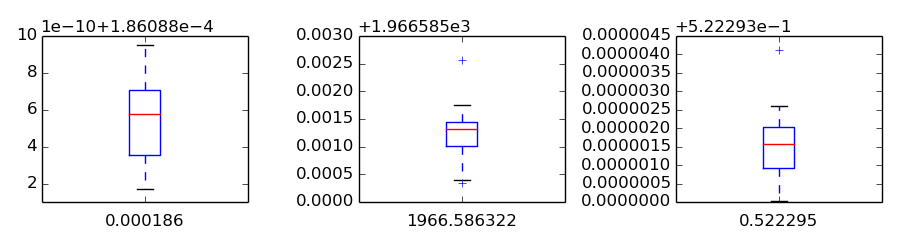
\includegraphics[width=\textwidth]{images/nm-summary.png}
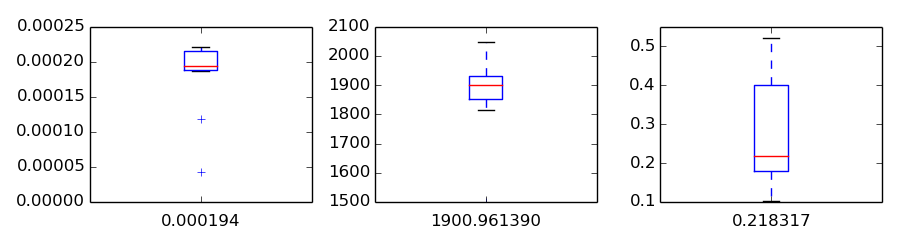
\includegraphics[width=\textwidth]{images/ga-summary.png}
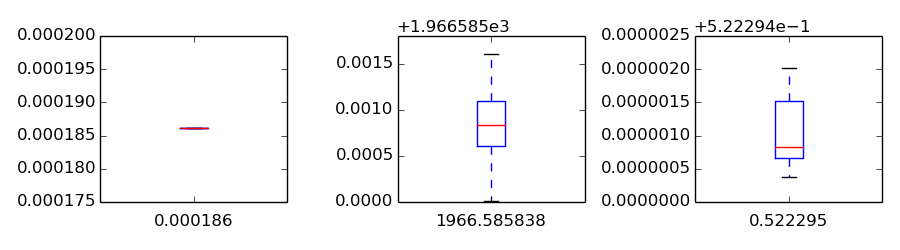
\includegraphics[width=\textwidth]{images/pso-summary.png}
\caption{Summary of 10 independent CoalHMM execution on the two-population isolation model using the three optimization methods.}
\label{fig:est-summary}
\end{figure}

The demographic parameters we use in this experiment are, 0.0002, 2083, and 0.5.  They are the split time of the two isolated populations, the coalescent rate, and the recombination rate, respectively.  These values are roughly recovered by CoalHMM.  We do recommend using PSO as it is the best tested and tuned optimization subroutine.

In summary, the following commands conduct a full simulation and estimation data analysis, and it summarizes the final results by creating box plots and printing the median estimate for each parameter.

{\scriptsize{}\begin{verbatim}
$ ./fsc251 -i input.par -n 1
$ ./arlequin2fasta.py input/input_1_1.arp 8000000
$ ./Jocx.py init . iso \
  ./input_1_1-sample_1-1_1.fasta \
  ./input_1_1-sample_2-2_1.fasta
$ ./Jocx.py run . iso pso 0.0001 1000 0.1 > pso-0.stdout
:
$ grep '500   1' pso-*.stdout > pso-summary.txt
$ ./box-plot-simple.py pso-summary.txt 3 pso-summary.png
\end{verbatim}}

The 1st command simulates a pairwise sequence alignment using the fastSIMCOAL2 program.  The 2nd command uses a custom script to convert the simulated alignment from the Arlequin format to the FASTA format.  The 3rd command prepares the ZipHMM directories using the FASTA sequences.  The 4th command executes CoalHMM's model inference and dumps the output to a file.  Potentially, multiple independent runs are dispatched and a HPC cluster is involved in this step.  The 5th command obtains the inference results from the output file.  The number 500 here is the maximum iteration count for this experiment, and the number 1 indicates the first particle in the last iteration.  Finally, the 6th command plots the parameters and presents the median estimates as the final results.

\section{Conclusions}

\todo[inline]{Write conclusions}


\bibliographystyle{spbasic}
\bibliography{references.bib}

\end{document}
